\section{Complete proof of the adaptive normal form}\label{app:normal}
We give a pathwise argument that allows arbitrary randomized adaptive auditing. A policy can use its own random seed, all previous audit observations, and any feedback that does not reveal a source change before it causes a failure or is audited. Audit outcomes disclose version equality; labels are rate-independent. The historical observation design is fixed and spans $m$ opportunities. A clean history is the unique history of unchanged values (up to rate-independent labels). Source hazards are constant throughout history and deployment.

\subsection{First-change lower bound}
Condition on the policy's internal random seed $R=r$. In the no-change world $h=0$, the history and all audit observations are deterministic, so the policy skips a fixed set $S_r\subseteq\{1,\ldots,T\}$; let $K_r=|S_r|$. For $t\in S_r$, consider the event $B_t$ that there is no change in the $m$ historical opportunities or deployment steps $1,\ldots,t-1$, and that a change occurs at step $t$. Its probability is $h(1-h)^{m+t-1}$, and no restriction is imposed on later changes.

On $B_t$, the controller has the same observable history as in the no-change world until its decision at $t$. Since it skips the check at $t$, it uses a stale value and fails. The events $\{B_t:t\in S_r\}$ are disjoint because they specify different first-change times. Hence, writing $q=1-h$,
\begin{equation}
 \Pp_h(F_T\mid R=r)\geq \sum_{t\in S_r}h q^{m+t-1}.
\end{equation}
For $0<h<1$ these summands decrease with $t$, so among sets with $K_r=k$ the last $k$ steps minimize the sum:
\begin{align}
 \sum_{t\in S_r} hq^{m+t-1}
 &\geq \sum_{t=T-k+1}^T hq^{m+t-1}\\
 &=q^{m+T-k}(1-q^k)=f_k(h).
\end{align}
The inequality extends by continuity to $h=0,1$, using $0^0=1$ when needed. Averaging over $R$ gives
\begin{equation}
 \Pp_h(F_T;\pi)\geq \Ee_R f_{K_R}(h).\label{eq:seedbound}
\end{equation}
This argument does not assume independent repeated failure events, nor that the policy stops after a failure. Only the first stale use matters.

\subsection{Attainment by a tail gate}
For $G_k$, any historical change is detected and triggers full auditing. Any change in the first $T-k$ deployment steps is detected before that step's action and also triggers full auditing. If neither event occurs, the final $k$ uses are unaudited and fail exactly when at least one of their source-change opportunities contains a change. History, prefix, and tail increments are independent, giving precisely
\begin{equation}
 \Pp_h(F_T;G_k)=q^{m+T-k}(1-q^k).
\end{equation}
The policy executes every action. At $h=0$, all checks are unchanged and $K=k$. Choosing $k$ before observing data according to the distribution of $K_R$ in Equation~\eqref{eq:seedbound} therefore weakly reduces risk at every $h$ without changing stable-instance saving.

\subsection{Two adjacent tail gates suffice}
For fixed $0<q<1$, extend $f_k(h)=q^n(q^{-k}-1)$ from integer $k$ to real $k\in[0,T]$, where $n=m+T$. This extension is convex. Its values at integer arguments therefore have nondecreasing successive slopes. Let $\overline f_h$ be the piecewise-linear interpolation through these integer values. It too is convex and satisfies $\overline f_h(j)=f_j(h)$ for every integer $j$.

For $x=\Ee K=k+a$ with integer $k=\lfloor x\rfloor$ and $a\in[0,1)$, Jensen's inequality gives
\begin{equation}
 \Ee f_K(h)=\Ee\overline f_h(K)\geq\overline f_h(x)=(1-a)f_k(h)+af_{k+1}(h).
\end{equation}
Crucially the same adjacent distribution attains this lower bound for \emph{every} $h$; it is not chosen after seeing the unknown hazard. Limits give the endpoints $h=0,1$. This proves the domination statement of Theorem~\ref{thm:normal}. Since the adjacent mixture is a valid policy, feasibility is both necessary and sufficient, establishing Equation~\eqref{eq:frontier}. The feasible set is closed and nonempty; the risk envelope is continuous and nondecreasing in $x$, so the maximum exists.

\subsection{Closed form, monotonicity, and rounding}
For real $0<x<n$, maximizing $q^{n-x}(1-q^x)$ over $q\in[0,1]$ yields
\begin{equation}
 q^x=\frac{n-x}{n},\qquad
 \sup_q q^{n-x}(1-q^x)
 =\frac{x}{n}\left(1-\frac{x}{n}\right)^{(n-x)/x}=\psi(x/n).
\end{equation}
The derivative of $\log\psi(s)$ is $-\log(1-s)/s^2>0$, proving strict monotonicity on $(0,1)$. The limiting values are zero and one. Applying Jensen directly to the smooth extension gives $\Pp_h(F_T)\geq q^{n-x}(1-q^x)$, hence $\psi(x/n)\leq\delta$ and Equation~\eqref{eq:continuous}.

For deterministic policies $x=k$ is an integer. The tail gate is feasible exactly when $\psi(k/n)\leq\delta$, so the optimum is the claimed floor. The adjacent randomized optimum is at least this integer and at most the real upper bound. If the upper bound is an integer it is itself attainable, so the rounding gap is zero; otherwise it is strictly less than one.

As $\delta\downarrow0$, $\psi(s)\sim s/e$, and therefore $s_\delta\sim e\delta$. The familiar first-order bound $e\delta(m+T)$ is a relaxation of the exact nonlinear expression. This asymptotic does not justify replacing the exact bound by $e\delta$ at arbitrary confidence levels.

\subsection{Numerically evaluating the exact frontier}
For $x=k+a$ with $0<a<1$, the adjacent risk as a function of $q$ is
\begin{equation}
 g(q)=(1-a)q^{n-k}+a q^{n-k-1}-q^n.
\end{equation}
Its interior stationary point solves
\begin{equation}
 a(n-k-1)+(1-a)(n-k)q-nq^{k+1}=0.\label{eq:derivative}
\end{equation}
For $k\geq1$ and $n-k-1>0$, the left side is concave, positive at zero and negative at one; its positive crossing is unique. For $k=0$, the maximizer is $q=(n-1)/n$ when $n>1$. For $n-k-1=0$, maximize $a+(1-a)q-q^n$ directly; if $n=1$, the maximum is $a$ at $q=0$. Integer $x$ uses the closed form. The implementation evaluates these cases with bracketed roots and includes endpoints. A second bracketed root finds the largest $x$ with risk at most $\delta$. The numerical implementation uses tolerances; the theorem is an exact mathematical statement, not a floating-point certificate for safety-critical code.

\section{Exposure geometry and calendar compilation}\label{app:exposure}
\subsection{Proof of Proposition~\ref{prop:exposure}}
For one source, a skipped use at $u_j$ is stale if there was a change after its last audit and at or before $u_j$. Collect these intervals over skipped uses. Split time into elementary intervals $(u_{j-1},u_j]$, with $u_0=0$. Such an interval is in the union exactly when use $j$ is skipped: if $j$ is audited, its preceding changes are corrected before any later use; if it is skipped, the interval is exposed immediately. Earlier exposed intervals remain part of the union even if an audit later corrects the value. Thus the union has size $\sum_j d_j s_j$.

No stale use occurs exactly when all change indicators in this union are zero. By temporal independence this has probability $(1-h_i)^{E_i}$ for source $i$. Independence across sources yields $\Pp_h(F_T^c)=\prod_i(1-h_i)^{E_i}$. In particular, a source with $E_i=0$ contributes a factor one even when $h_i=1$.

An audit strictly between two consecutive required uses can be moved to the latter use. There is no intervening required action, and the later audit removes at least as many changes before the next action. If there is already an audit there, the earlier audit can simply be removed. This argument uses no resource capacity, no time-dependent cost, and no informative value for intermediate audits in a fixed-calendar policy. It does not prove that off-use audits are redundant for general learning policies.

\subsection{Optimal per-source calendar under a cap}
For a fixed group budget $\delta_G$, Theorem~\ref{thm:gate} requires $E_i\leq r_{\delta_G}m_i$ separately for every source. If every check of source $i$ has the same cost $c_i$, maximizing its saved cost is equivalent to maximizing the number of skipped checks. Sort $d_{ij}$ in increasing order. For any $k$, the sum of the $k$ shortest gaps is no greater than the exposure of any $k$ skipped uses. Consequently the longest feasible prefix of this ordering is optimal. Stable sorting resolves ties without randomness. The methods allow arbitrary source costs but not arbitrary within-source time-varying costs; the latter require a knapsack solver instead of sorting.

\subsection{Known-rate knapsack baseline}
With known rates, the risk constraint is $\sum_{i,j}\lambda_i d_{ij}s_{ij}\leq-\log(1-\delta)$. For integer costs, the implementation keeps the minimum log-risk required to save each possible total integer cost, then backtracks the largest feasible saving. This is exact in the finite instances, modulo floating-point arithmetic. It avoids a risk-grid relaxation. It is optimal among fixed calendars, not among adaptive policies using audit outcomes. Its true-rate information advantage is explicitly labeled in every comparison.

\section{Proofs for joint gates and conditional guarantees}\label{app:joint}
\subsection{Sharp marginal certificate}
Let $C_G$ be the event that every group history is clean. On $C_G^c$ every required use is audited, so there is no stale-use failure. On $C_G$, the calendar is fixed independently of future changes. Temporal and source independence give
\begin{equation}
 \Pp_h(F_G)=\Pp_h(C_G)\Pp_h(F_G\mid C_G)
 =e^{-x}(1-e^{-y}),
 \quad x=\sum_i m_i\lambda_i,\quad y=\sum_i E_i\lambda_i.
\end{equation}
For $0<r<\infty$, $y\leq rx$ and therefore
\begin{equation}
 \Pp_h(F_G)\leq e^{-x}(1-e^{-rx}).
\end{equation}
Differentiating with respect to $x\geq0$ gives a unique maximum at $x^*=\log(1+r)/r$, with value
\begin{equation}
 e^{-x^*}(1-e^{-rx^*})=(1+r)^{-1/r}\frac{r}{1+r}=\phi(r).
\end{equation}
Choose $j$ with $E_j/m_j=r$, set $\lambda_j=\log(1+r)/E_j$, and set all other rates to zero. Then $x=x^*$ and $y=rx^*$, proving attainment. If every exposure is zero, the risk is zero. If a source has positive exposure and no history, set its hazard to one and all others to zero; the risk is one. This handles the endpoint cases and proves Theorem~\ref{thm:gate}.

\paragraph{Connection to the single-source normal form.}
A tail gate with $k$ skipped deployment uses has total tested span $m+T-k$ and future exposure $k$. Its ratio is $r=k/(m+T-k)$, so $\phi(r)=\psi(k/(m+T))$. Thus the clean-history certificate and the adaptive normal form use the same risk function, but different policy classes: one folds prefix audits into a history; the other starts from an arbitrary adaptive policy and proves a dominating form.

\subsection{Proof of Proposition~\ref{prop:conditional}}
Let $c=-\log(1-\rho)>0$. A dirty history triggers the all-audit calendar with conditional risk zero. A clean history triggers the prescribed calendar, whose risk exceeds $\rho$ exactly when $y=\sum_iE_i\lambda_i>c$. For any fixed $h$ in this unsafe region, the probability of issuing that unsafe calendar is $e^{-x}$. Since $y\leq rx$, it is at most $e^{-c/r}$. Conversely choose a maximizing-ratio source and let $y\downarrow c$ from above. This makes $x=y/r$ and $e^{-x}\uparrow e^{-c/r}$. Hence
\begin{equation}
 \sup_{h:\,\risk_h(A)>\rho}\Pp_h(C_G)=e^{-c/r}.
\end{equation}
The requirement that this probability be at most $\alpha$ is equivalent to Equation~\eqref{eq:pac}. The strict risk inequality does not change the supremum. The result concerns this clean-history gate, not every possible conditional-certificate procedure.

\begin{figure}[t]
\centering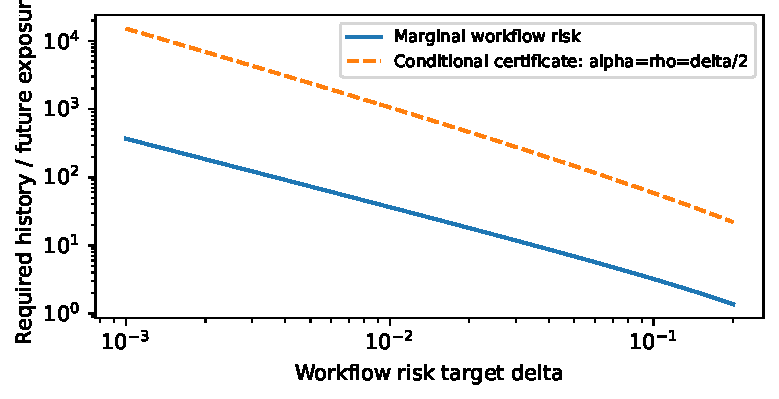
\includegraphics[width=.9\linewidth]{figures/evidence.pdf}
\caption{Historical span required per unit of future exposure. The conditional guarantee takes $\alpha=\rho=\delta/2$ and is intentionally stronger than a marginal workflow guarantee. These are evidence-span requirements, not numbers of endpoint audits.}\label{fig:evidence}
\end{figure}

For $\alpha=\rho=\delta/2$, the conditional requirement scales as approximately $2E\log(2/\delta)/\delta$. The marginal requirement scales as $E/(e\delta)$. This separation is a comparison between different guarantees; it is not a lower bound asserting that every marginally safe algorithm needs a logarithm. Indeed Theorem~\ref{thm:normal} provides the exact stable-instance result without that logarithm.

\subsection{Fixed-gap binomial confidence baseline}
If audits are separated by a fixed gap $d$ and $n$ disjoint windows are observed, the number $K$ of windows with at least one change is binomial with probability $p=1-(1-h)^d$. The one-sided Clopper--Pearson upper endpoint is
\begin{equation}
 p^+=\begin{cases}
 \operatorname{Beta}^{-1}(1-\alpha_i;K+1,n-K),&K<n,\\
 1,&K=n.
 \end{cases}
\end{equation}
Transform it to $h^+=1-(1-p^+)^{1/d}$. In particular, $p^+=1$ must map to $h^+=1$, not a floating-point clipped smaller number. With $\sum_i\alpha_i\leq\alpha$, all true rates are covered simultaneously with probability at least $1-\alpha$. A calendar selected using any of these same rate bounds and satisfying their worst-case future risk $\rho$ therefore has marginal risk at most $\alpha+(1-\alpha)\rho$.

The calendar can be data-dependent because rate coverage is simultaneous across its source coordinates. This argument does not allow arbitrary stopping times for the observations, repeated use of a fixed-sample bound, or pilot/validation leakage. We used fixed sample counts and gaps. Our separate calibration experiment reports both coverage violations and actual unsafe-calendar decisions, since the latter need not occur every time one bound misses.

\section{Composition, optimization, and selection}\label{app:partition}
\subsection{Proof of Theorem~\ref{thm:compose}}
For fixed disjoint groups, $F_G$ depends only on the histories and deployment change indicators of the sources in $G$. The events are therefore independent, even if sources are required by the same action. Hence $\Pp_h(F_T)=1-\prod_G(1-\Pp_h(F_G))$. Each group term is bounded by $\phi(r_G)$. Conversely the separate least-favorable hazard vectors in Theorem~\ref{thm:gate} can be combined because the groups use disjoint coordinates. This attains the displayed worst case simultaneously.

The saving contributed by group $G$ is $S_G\1\{C_G\}$; its expectation is $S_Ge^{-\sum_{i\in G}m_i\lambda_i}$. Summing proves Equation~\eqref{eq:utility}. No independence is needed for linearity of the saving expectation, but independence is needed for the displayed failure product and the group acceptance formula.

Now condition on an independent pilot realization $Z=z$. The selected groups, schedules, and log budgets are deterministic functions of $z$ (or of additional independent algorithmic randomness). The gate histories and future increments still have the original source process laws at the true fixed $h$. The just-proved risk inequality therefore holds conditionally on $z$, regardless of whether $z$ estimates $h$ well. Averaging over $Z$ preserves the upper bound $\delta$. This is an independent-data selection argument, not a claim that the pilot makes the true rates known.

\subsection{Optimality of the restricted dynamic program}
Fix a source order, grid size $L$, and nonnegative predicted hazards. For a contiguous group $[a,b)$ and budget $z$, the optimal source calendars follow the shortest-gap rule. Their predicted expected saving is $v(a,b,z)$. Any allowed partition of the first $b$ ordered sources has a final group $[a,b)$ and spends some $w\leq z$ units on it. Its preceding groups form an allowed solution for the first $a$ sources with at most $z-w$ units. Conversely any such preceding solution and last group form an admissible partition. Taking maxima proves Equation~\eqref{eq:dp} by induction on $b$.

The base values $V(0,z)=0$ permit unused budget. A zero-budget group skips no checks and contributes zero utility; thus every source can be included even when it should always be audited. There are $O(NL)$ dynamic-programming states and $O(NL)$ predecessors per state, giving $O(N^2L^2)$ time. Group acceptance factors and skip-value sums can be calculated using prefix sums after per-source menus are formed. The implementation stores backpointers to recover the actual partition and independently recomputes its certificate before returning it.

The state space does not contain noncontiguous groups in the chosen order, nongrid budget allocations, or outcome-dependent post-gate selection. The optimality claim must not be generalized to those classes. The order and predicted utility can be poor when the pilot contains few observed changes. Table~\ref{tab:main} and the long-history negative results illustrate the resulting performance loss.

\subsection{A post-selection counterexample}
Take $N$ identical independent sources and select the first clean history, if any, reusing only that source for an exposure of $E$; if none is clean, audit everything. At the fixed underlying rate $h$, define $a=(1-h)^m$ and $b=1-(1-h)^E$. A preselected source has risk $ab$. The selected source's future is independent of all histories and still has failure probability $b$, while the probability that some source is selected is $1-(1-a)^N$. Thus actual risk is
\begin{equation}
 [1-(1-a)^N]b.\label{eq:selectionfailure}
\end{equation}
For $m=1000$, $E=145$, choose the least-favorable scalar rate $h=1-\exp[-\log(1+E/m)/E]$. The fixed-source worst risk is $.04977456$, but Equation~\eqref{eq:selectionfailure} gives $.124305$ at $N=8$. Relabeling the selected source as a fixed group after the fact does not repair the guarantee.

\subsection{Correlated sources and rate shift}
For a separate counterexample, let all sources share the same Bernoulli change sequence. Give them the same historical interval of length $m$, so the all-clean event has probability $q^m$, not $q^{Nm}$. Construct fixed calendars with pairwise disjoint future exposed intervals of length $E$ each, with source-specific audits immediately before each interval. The actual probability of some stale use after acceptance is
\begin{equation}
 q^m(1-q^{NE}),
\end{equation}
whose supremum is $\phi(NE/m)$. The independent-source formula would incorrectly give $\phi(E/m)$. This construction is deliberately outside the paper's model; it demonstrates why source independence is not a cosmetic assumption.

A single-source time-shift example instead keeps historical hazard $h_0$ and increases the deployment hazard to $h_1$. Actual risk is $(1-h_0)^m[1-(1-h_1)^E]$. Setting $h_0$ to the stationary least-favorable rate and $h_1=2h_0$ gives $.093284$ for the same $m,E$. Our stationary certificate cannot be reused under this shift.

\begin{figure}[t]
\centering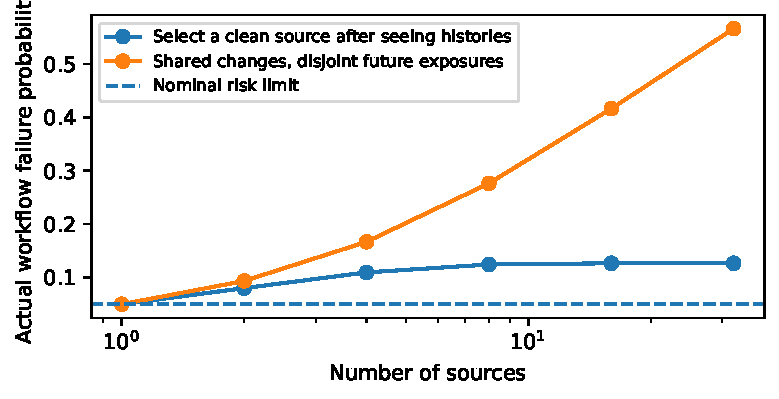
\includegraphics[width=.9\linewidth]{figures/misspecification.pdf}
\caption{Constructive violations of assumptions, evaluated exactly. Selecting a source after observing the gate histories, or sharing change events across sources, can exceed the nominal 5\% risk limit. These curves are not performance predictions for a deployment.}
\end{figure}

\section{Experimental protocol and additional results}\label{app:experiments}
\subsection{Data generation and accounting}
Every scene has $N=8$ sources and horizon $T=200$. Costs are $(1,1,2,2,1,1,2,2)$, so 32 checks per source cost 384. Four sources have four disjoint bursts of eight consecutive uses; burst starts are sampled from a ten-step-spaced grid. The other four have 32 distinct uniformly sampled use times. The rates before random perturbation are
\begin{align*}
 h^{\rm stable}&=(0,0,1,1,2,2,3,3)\cdot10^{-5},\\
 h^{\rm mixed}&=(0,10^{-5},10^{-5},2\cdot10^{-5},2\cdot10^{-5},3\cdot10^{-5},.001,.003),\\
 h^{\rm active}&=(1,2,3,4,5,6,8,10)\cdot10^{-4}.
\end{align*}
Each nonzero rate is multiplied by an independent uniform factor in $[.8,1.2]$. Ten fixed seeds generate scenes and pilots. The history span is separately set to $200$, $1000$, or $5000$ for every source. Within a scene, methods share the same exogenous use pattern and rate vector.

The independent pilot has $n_p=64$ windows of length $d_p=50$ per source. If $K_i$ windows contain changes, its plug-in hazard is $\widehat h_i=1-(1-K_i/n_p)^{1/d_p}$. These estimates only affect the grouping order and predicted utility. They are not used as confidence bounds. For the CP comparator, a second, independent history has ten windows of length $m/10$. Its confidence allocation is $.025/8$ per source and its future-risk budget is $.025$. No pilot or history parameter is tuned using hidden test changes.

For clean gates, risk and cost are analytically averaged over the second history; a history is clean precisely when none of its windows contains a change. A single observation at the beginning of this span, followed by the common time-zero observation, is sufficient to test cleanliness under nonreversion. The extra endpoint costs 12 weighted audits; intermediate observations add no information about the \emph{all-clean} event. CP uses the intermediate counts and is charged 120. Pilot acquisition costs 768 weighted audits and span 3200. These are fixed experimental choices, not an optimized evidence-acquisition policy. The rate-informed references receive true rates for free and are not cost-comparable deployed learners.

\subsection{Oracle and validation coverage}
The 1,856 adaptive policies are all deterministic binary audit trees at horizons 1 through 4. A skip provides no change observation; an audit has clean and changed successors. We enumerate all binary source-change sequences for each policy and aggregate failure probabilities by polynomial coefficients in $h$. Derivative roots and interval endpoints yield an independent numerical maximizer of this polynomial. Grouping policies by stable skip count verifies both the lower envelope and attainment by a tail gate.

For randomized-policy validation, ten linear programs mix the full policy sets at horizons 3 and 4. They enforce risk bounds on a grid of 121 hazard values \emph{and} the exact adjacent-mixture least-favorable hazard. The resulting upper relaxation matches the analytic optimum to within $8\times10^{-13}$. It remains a finite numerical check, not a proof of continuum feasibility. Sixty independently generated two-source tiny calendars enumerate a total of 71,808 change worlds, directly updating version counters and cache states. Their exact weighted failure frequencies match Equation~\eqref{eq:exposure} to numerical tolerance.

The 300 joint and 300 partition witnesses use independently sampled histories, exposures, and source counts up to six. Each checks that the explicit worst-case parameter attains the closed form. Unit tests also exhaust tiny skip subsets, knapsack solutions, and five small ordered-partition problems. All 83 tests passed locally. The suite checks zero exposure, zero history, hazard one, all-changed CP histories, and very small clean-history probabilities. Assertions use numerical tolerances; none is a machine-checked formal proof.

\subsection{Explicit workflow simulation}
For each of three regimes, three history spans, and three methods (single group, separate sources, and pilot grouping), the simulator runs 2,000 independent workflows: 54,000 total. It samples clean histories, then simulates every source change, audit update, and required use by version counters. Identical random seeds couple exogenous events across methods where possible, but controllers never access hidden states. Whole workflows, not their action steps, are independent sampling units. Figure~\ref{fig:rollouts} compares observed failure frequency with analytic probability. The largest absolute discrepancy is about $.0059$; the paper's rare-event claims rely on the mathematical model, not on absence of observed failures.

\begin{figure}[t]
\centering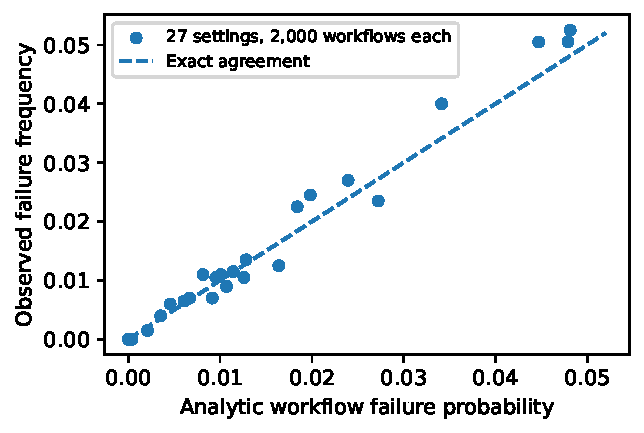
\includegraphics[width=.8\linewidth]{figures/rollout_check.pdf}
\caption{Independent state-simulator check of the risk calculation. Each point uses 2,000 complete workflows. This is a mechanism validation, not a claim that small samples establish extremely small failure probabilities.}\label{fig:rollouts}
\end{figure}

The CP calibration uses four sources with 16 uses each, history spans $100$, $1000$, and $5000$, two rate scales, and 200 independent histories per combination: 1,200 datasets. We separately record whether any rate bound misses and whether the selected calendar has actual conditional risk above $.025$. No unsafe conditional calendar was observed in this run. This observation is weaker than a formal universal claim; the valid fixed-sample guarantee follows from the confidence construction, subject to the model assumptions.

\subsection{Additional grouping curves and weaker baselines}
Figures~\ref{fig:stablegroups} and~\ref{fig:activegroups} complement the mixed-rate main plot. The pilot frequently sees no changes at low rates, so many estimated hazards tie. At long historical spans, grouping errors become expensive because one genuinely active source suppresses reuse for its entire group. Rate-informed grouping has a better predicted objective because its predictions are correct, but is still restricted to an ordered partition and a log-budget grid.

\begin{figure}[t]
\centering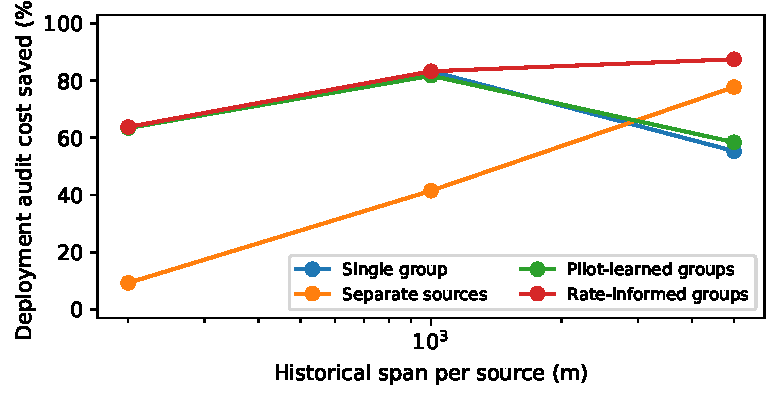
\includegraphics[width=.9\linewidth]{figures/grouping_stable.pdf}
\caption{Stable regime. Large groups are effective with intermediate spans; separate sources can outperform a noisy learned partition with longer histories.}\label{fig:stablegroups}
\end{figure}
\begin{figure}[t]
\centering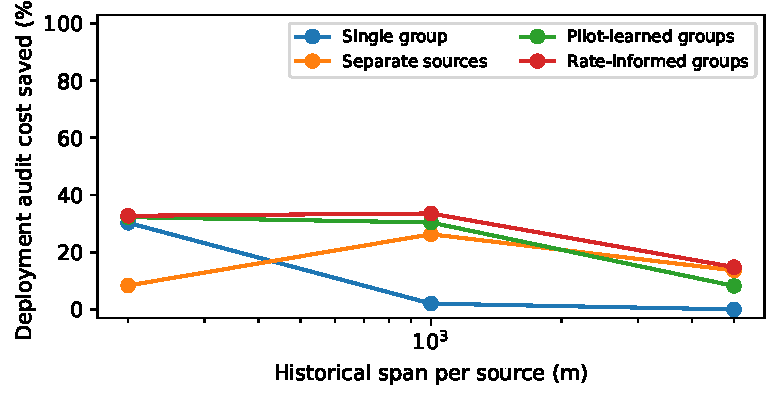
\includegraphics[width=.9\linewidth]{figures/grouping_active.pdf}
\caption{Active regime. A single all-clean gate has rapidly collapsing acceptance probability as the historical span grows. Even pilot grouping may lose to separate sources.}\label{fig:activegroups}
\end{figure}

The point-estimated knapsack and global expiration-time comparators spend risk according to pilot rates without a confidence correction. Their low audit costs do not imply uniform reliability. All their actual risks, including violations, are retained in \texttt{workflow\_results.csv}; they are not dropped because they fail certification. The global expiration-time comparator is selected from all integer expiration times up to $T+1$ using nominal risk, not hidden actual risk. Equal-source groups are a strong certified baseline that requires no learned partition or pilot acquisition.

\subsection{Reproduction commands and scope of artifacts}
From a clean Python environment in the repository root:
\begin{minipage}{\linewidth}
\begin{verbatim}
python -m pip install -r requirements.txt
python -m pytest -q
python experiments/run_all.py
python experiments/additional_checks.py
python experiments/make_figures.py
make paper
\end{verbatim}
\end{minipage}
The first two experiment scripts produce 12 CSVs; the figure script produces vector PDF figures, PNG previews, the main table, and a headline JSON. CSV hashes are recorded in \path{results/manifest.json}. Scientific results should reproduce numerically across supported library versions; exact bytes are checked when the runtime is identical. Wall-clock metadata are not deterministic and are not scientific outcomes. The experiments require only CPU numerical libraries, not a GPU, model weights, paid APIs, or downloads. Fetching the conference style, when absent, is a separate formatting step and has no role in the experiments.

\section{Claim boundaries and unresolved extensions}\label{app:boundaries}
\paragraph{What is established.}
Theorem~\ref{thm:normal} concerns every randomized adaptive policy in the single-source, every-step-use model, but optimizes only its stable-instance saving. Theorem~\ref{thm:gate} is an exact worst-case risk characterization for the stated fixed-calendar clean-history gate. Theorem~\ref{thm:compose} composes disjoint source groups; the dynamic program is exact only for its ordered-partition and budget-grid objective. The experiments check finite mechanisms and implementation consistency.

\paragraph{What is not established.}
The paper does not prove the optimal expected cost at arbitrary nonzero hazards, optimal online multi-source revalidation, or minimax-optimal pilot allocation. It does not provide a safety guarantee after conditioning on every admitted history, under arbitrary source dependence, under hazard drift, after adaptive stopping of a fixed-sample history, or for repeated workflows without risk accounting. The workflow semantics treat stale versions as action failure by design. A real task may tolerate some stale facts and fail for reasons unrelated to memory; these require different loss and observation models.

\paragraph{Why more data can appear harmful.}
For a fixed clean-history gate, more history simultaneously increases $E\leq r_\delta m$ and decreases the probability of acceptance. A policy allowed to select a shorter \emph{prespecified} subhistory can avoid some losses, but choosing the most favorable clean subhistory after seeing all outcomes is a selection problem. Our comparisons hold the historical window fixed and reveal that gate-specific tradeoff. They do not prove that access to additional data reduces the optimal attainable performance.

\paragraph{Amortization and future directions.}
Historical evidence acquired for other purposes can make reuse worthwhile, but purchasing a pilot for one short workflow may not. Reusing a pilot with new, properly specified gate histories preserves per-workflow safety; a global multi-workflow target needs its own risk allocation or joint analysis. Optimal evidence acquisition and outcome-rich testing rules remain outside our guarantees.
